
% compile using 
%   pdflatex --shell-escape
% to enable using gnuplot
\documentclass[dvipsnames,colorlinks=true,urlcolor=green]{beamer}
%\documentclass[dvipsnames,colorlinks=true,urlcolor=green]{article}
\usepackage[latin1]{inputenc}
\usetheme{Warsaw}
\usepackage{colortbl}

%\useoutertheme{infolines}
\useoutertheme{default}

%\useoutertheme{sidebar}
%\usetheme{Singapore}
%\usetheme{compatibility}
%\useinnertheme{rounded}
\usepackage{pgf}
\usepackage{amsmath,amssymb,amsxtra}
\usepackage{amsthm}
\usepackage{hyperref}

\usepackage{beamerfoils}
%\usepackage{beamerarticle}


\usepackage{tikz}
\usepackage{animate}
\usetikzlibrary{calc,arrows,backgrounds,positioning,fit}

% get less space before and after equations
\setlength{\abovedisplayskip}{5pt}
\setlength{\belowdisplayskip}{10pt}
\setlength{\abovedisplayshortskip}{5pt}
\setlength{\belowdisplayshortskip}{10pt} 

\newcounter{m}
\setcounter{m}{0}
\newcounter{c}
\setcounter{c}{0}


\mode<handout>{\usetheme{Warsaw}}

\pgfdeclareimage[height=3cm,width=3cm]{logo}{watsonlogo}
\MyLogo{\pgfuseimage{logo}}
%\usebeamertemplate*{logo}


\definecolor{IBMBlue}{rgb}{0,0,0.7}
\definecolor{m1}{rgb}{0.1,0.1,0.9}
\definecolor{m2}{rgb}{0.8,0.2,0.2}

\parindent 0pt		  % sets leading space for paragraphs




\def\trace{\mathop{\mathrm{trace}}}
\newcommand{\N}{\mathcal{N}}
\newcommand{\R}{\mathbb{R}}
\newcommand{\Z}{\mathbb{Z}}
\renewcommand{\L}{\mathcal{L}}
\newcommand{\F}{\mathcal{F}}
\newcommand{\Tr}{\mathrm{Tr}}
\newcommand{\half}{\frac{1}{2}}
\newcommand{\diag}{\mathrm{diag}}
\newcommand{\Var}{\mathrm{Var}}
\newcommand{\dd}[1]{\;\mathrm{d#1}}
\def\myvec{\mathrm{vec}}



\def\L{{\cal L}}
\def\logdet{\mathrm{log\;det}}
\def\det{\mathop{\mathrm{det}}}

\def\va{\mathbf{a}}
\def\vb{\mathbf{b}}
\def\vg{\mathbf{g}}
\def\vp{\mathbf{p}}
\def\vr{\mathbf{r}}
\def\vs{\mathbf{s}}
\def\vv{\mathbf{v}}
\def\vw{\mathbf{w}}
\def\vx{\mathbf{x}}
\def\vy{\mathbf{y}}
\def\vz{\mathbf{z}}
\def\vmu{\boldsymbol{\mu}}
\def\vxi{\boldsymbol{\xi}}
\def\vphi{\boldsymbol{\phi}}
\def\vpsi{\boldsymbol{\psi}}
\def\vtheta{\boldsymbol{\theta}}
\def\mDelta{\boldsymbol{\Delta}}
\def\mLambda{\boldsymbol{\Lambda}}
\def\mSigma{\boldsymbol{\Sigma}}
\def\mA{\mathbf{A}}
\def\mB{\mathbf{B}}
\def\mC{\mathbf{C}}
\def\mD{\mathbf{D}}
\def\mE{\mathbf{E}}
\def\mF{\mathbf{F}}
\def\mG{\mathbf{G}}
\def\mH{\mathbf{H}}
\def\mI{\mathbf{I}}
\def\mK{\mathbf{K}}
\def\mL{\mathbf{L}}
\def\mP{\mathbf{P}}
\def\mQ{\mathbf{Q}}
\def\mR{\mathbf{R}}
\def\mS{\mathbf{S}}
\def\mT{\mathbf{T}}
\def\mV{\mathbf{V}}
\def\mW{\mathbf{W}}
\def\mX{\mathbf{X}}
\def\mY{\mathbf{Y}}
\def\mZ{\mathbf{Z}}
\def\m0{\mathbf{0}}
\usepackage[british]{babel}
\usepackage{graphicx,hyperref,ru, url}

% The title of the presentation:
%  - first a short version which is visible at the bottom of each slide;
%  - second the full title shown on the title slide;
\title[An Automatic Matrix Differentiation Library]{
  An Automatic Matrix Differentiation Library}

% Optional: a subtitle to be dispalyed on the title slide
%\subtitle{IBM T.J. Watson Research Center}

% The author(s) of the presentation:
%  - again first a short version to be displayed at the bottom;
%  - next the full list of authors, which may include contact information;
\author[Suyang Zhu, Peder Olsen and Prabhanjan Kambadur]{
  Suyang Zhu, Peder Olsen and Prabhanjan Kambadur \\\medskip
  }

% The institute:
%  - to start the name of the university as displayed on the top of each slide
%    this can be adjusted such that you can also create a Dutch version
%  - next the institute information as displayed on the title slide
\institute[IBM]{IBM T.J. Watson Research Center}

% Add a date and possibly the name of the event to the slides
%  - again first a short version to be shown at the bottom of each slide
%  - second the full date and event name for the title slide
\date[August 8 2014]{
  August 8th, 2014}

\begin{document}

\begin{frame}
  \titlepage
\end{frame}

\begin{frame}
  \frametitle{Outline}

  \tableofcontents
\end{frame}

%\section{Introduction}
\section{Matrix Differentiation}

\begin{frame}
\frametitle{Terminology}
Classical calculus:
\begin{itemize}
\item {scalar-scalar functions} ($\color{m1}f:\R\rightarrow\R$)
\item scalar-vector functions ($\color{m1}f:\R^d\rightarrow\R$).  
\end{itemize}
Matrix calculus:
\begin{itemize}
\item \alert{scalar-matrix functions} ($\color{m1}f:\R^{m\times
  n}\rightarrow\R$)
\item \alert{matrix-matrix functions}
($\color{m1}f:\R^{m\times
  n}\rightarrow\R^{k\times l}$).
\end{itemize}
Note:
\begin{enumerate}
\item Derivatives of scalar-matrix functions requires derivatives of
  matrix-matrix functions (why?)
\item Matrix-matrix derivatives should be computed implicitly wherever
  possible (why?)
\end{enumerate}
\end{frame}


\begin{frame}
\frametitle{Optimizing Scalar-Matrix Functions}
Useful quantities for optimizing a scalar-matrix function
$$\color{m1}f(\mX):\R^{d\times d}\rightarrow\R$$

\vspace{-1cm}
\begin{itemize}
\setlength{\itemsep}{0pt}
\setlength{\parskip}{0pt}
\setlength{\parsep}{0pt}
\setlength{\partopsep}{0pt}
\setlength{\topsep}{0pt}
 \item The gradient is a matrix--matrix function:
$$\color{m1}f'(\mX):\R^{d\times d}\rightarrow\R^{d\times d}.$$
\item The Hessian is also a matrix-matrix function: 
$$\color{m1}f''(\mX):\R^{d\times d}\rightarrow\R^{d^2\times d^2}.$$
\end{itemize}

\vspace{-.5cm}
Desiderata:  The derivative of a matrix--matrix function should be a matrix, so
that we can directly use it to compute the Hessian.
\end{frame}

\begin{frame}
\frametitle{Optimizing Scalar-Matrix Functions (continued)}
Taking the scalar--matrix
derivative of 
$$\color{m1}f(\mG(\mX))$$  
will require the information in the matrix--matrix derivative
$$\color{m1}
\frac{\partial\mG}{\partial\mX}.
$$
Desiderata: The derivative of a matrix-matrix function should be a
matrix, so that a convenient chain-rule can be established.
\end{frame}

\begin{frame}
\frametitle{The vec Operator}
For a matrix $\color{m1}A\in \R^{m\times n}$ we define $\color{m1} vec(A)$  to be the column-stacked vector of $\color{m1}A$
$$\color{m1}
vec(A) = 
\begin{pmatrix} 
a_{11} \\
a_{12} \\
\vdots \\
a_{1n} \\
a_{21} \\
\vdots \\
a_{mn} \\
\end{pmatrix}.
$$
\end{frame}

\begin{frame}
\frametitle{The Scalar-Matrix Derivative}
For $\color{m1}f:\R^{m\times n}\rightarrow\R$ the scalar-matrix derivative is defined
to be: 
$$\color{m1}
\frac{\partial f}{\partial \mX} \stackrel{\mathrm{def}}{=} 
\begin{pmatrix} 
\frac{\partial f}{\partial {x_{11}}} &
\frac{\partial f}{\partial {x_{12}}} & \cdots & 
\frac{\partial f}{\partial {x_{1n}}}\\
\frac{\partial f}{\partial x_{21}} &
\frac{\partial f}{\partial x_{22}} & \cdots & 
\frac{\partial f}{\partial x_{2n}}\\
\vdots & \vdots & \ddots & \vdots \\
\frac{\partial f}{\partial x_{m1}} &
\frac{\partial f}{\partial x_{m2}} & \cdots & 
\frac{\partial f}{\partial x_{mn}}
\end{pmatrix}.
$$
\end{frame}
\begin{frame}
\frametitle{The Matrix-Matrix Derivative}
For $\color{m1}f:\R^{m\times n}\rightarrow\R^{k\times l}$ the matrix--matrix derivative is defined
to be: 
$$\color{m1}
\frac{\partial \mF}{\partial \mX} \stackrel{\mathrm{def}}{=} 
\frac{\partial
  \myvec(\mF^\top)}{\partial \myvec^\top(\mX^\top)} = 
\begin{pmatrix} 
\frac{\partial \alert<3>{f_{11}}}{\partial \alert<2>{x_{11}}} &
\frac{\partial f_{11}}{\partial \alert<2>{x_{12}}} & \cdots & 
\frac{\partial f_{11}}{\partial \alert<2>{x_{mn}}}\\
\frac{\partial \alert<3>{f_{12}}}{\partial x_{11}} &
\frac{\partial f_{12}}{\partial x_{12}} & \cdots & 
\frac{\partial f_{12}}{\partial x_{mn}}\\
\vdots & \vdots & \ddots & \vdots \\
\frac{\partial \alert<3>{f_{kl}}}{\partial x_{11}} &
\frac{\partial f_{kl}}{\partial x_{12}} & \cdots & 
\frac{\partial f_{kl}}{\partial x_{mn}}
\end{pmatrix}.
$$
\onslide<4>{
Note that the matrix--matrix derivative of a scalar--matrix function
is not the same as the scalar--matrix derivative:
$$\color{m1}
\frac{\partial\;\mbox{mat}(f)}{\partial\mX} = \myvec^\top\left(
\left( \frac{\partial f}{\partial\mX}\right)^\top
\right) .
$$}
\end{frame}

\begin{frame}
\frametitle{Basic Differentiation Identitities}
Let $\color{m1}\mX\in\R^{m\times n}$.
\begin{itemize}
\item \textbf{Identity}: $\color{m1}\mF(\mX)=\mX$, $\color{m1}\mF'(\mX)=\mI_{mn}$
\item \textbf{Chain Rule}: 
$\color{m1}\mF(\mX)=\mG(\mH(\mX)),\quad\mF'(\mX)=\mG'(\mH(\mX))\mH'(\mX)$
\item \textbf{Product Rule}: 
$$\color{m1}\mF(\mX)=\mG(\mX)\mH(\mX),\quad\mF'(\mX)=(\mI\otimes\mH^\top(\mX))\mG'(\mX)+(\mG(\mX)\otimes\mI)\mH'(\mX)$$
\end{itemize}

Assume $\color{m1}\mX\in\R^{m\times m}$ is a square matrix.
\begin{itemize}
\item \textbf{Square:}
$\color{m1}\mF(\mX)=\mX^2$, $\color{m1}\mF'(\mX)=\mI_m\otimes\mX^\top+\mX\otimes\mI_m$.
\item \textbf{Inverse:} $\color{m1}\mF(\mX)=\mX^{-1}$, $\color{m1}\mF'(\mX)=-\mX^{-1}\otimes\mX^{-\!\top}$.
\item \textbf{Integer Power:} $\color{m1}\mF(\mX)=\mX^k$,
  $\color{m1}\mF'(\mX)=\sum_{i=0}^{k-1}\mX^i\otimes(\mX^{k-1-i})^{\top}$.
\end{itemize}
\end{frame}

\begin{frame}
\frametitle{Scalar-Matrix Differentiation}
First some simple identities:
$$\color{m1}
\begin{array}{ll}
f(\mX)=\trace(\mA\mX) & \qquad f'(\mX) = \mA^\top \\
f(\mX)=\logdet(\mX) & \qquad f'(\mX) = \mX^{-\!\top}
\end{array}
$$
Then the chain rule for more general expressions:
{\color{m1}
\begin{eqnarray*}
\myvec\left(\left(\frac{\partial}{\partial
  \mX}\logdet(\mG(\mX))\right)^\top\right) &=&
\left(\frac{\partial\mG}{\partial\mX}\right)^\top\myvec\left(\left(\mG(\mX)\right)^{-1}\right)\\
\myvec\left(\left(\frac{\partial}{\partial
  \mX}\trace(\mG(\mX))\right)^\top\right) &=&
\left(\frac{\partial\mG}{\partial\mX}\right)^\top\myvec(\mI)
\end{eqnarray*}}

$\color{m1} \frac{\partial \mG}{\partial \mX}$ can be written as $\color{m1}\sum_{i} \mA_{i} \otimes \mB_{i}$. Thus $\color{m1} \frac{\partial \mG}{\partial \mX}vec(\mY)$ can be compute efficiently.
\end{frame}


\begin{frame}
\frametitle{Forward Mode Differentiation}
\centerline{Compute $\color{m1}f(\mX)=\trace(\mF(\mX))=\trace(((\mI+\mX)^{-1}\mX^\top)\mX)$}
\begin{center}
\begin{tikzpicture}
[scale=.7,transform shape,
matrix/.style={rectangle,draw=black,fill=blue!20,thick},
operation/.style={circle,draw=black,fill=red!20,thick},
arrow/.style={->,thick}]
\node[matrix] (F) {$\trace(\mF(\mX))$};
\node[left=5cm of F] (upperLeft) { };
\node[right=2cm of F] (upperRight) { };
\node [right,left=2pt of F]  (tmpF) at (F.west)
{
\only<7->{$\color{blue}f=\trace(\mT_5)$}
};\node[operation] (root) [below=of F] {$\times$}
edge [arrow] (F);
\node [right,left=2pt of root] (tmpRoot)
{
\only<6->{$\color{blue}\mT_5=\mT_4*\mX$}
};
\node[operation] (t4) [below left=of root] {$\times$}
edge [arrow] (root);
\node [left,align=center,red] (tmp4) at (t4.west)
{
\only<5->{$\color{blue}\mT_4=\mT_2*\mT_3$}
};
\node[matrix] (x3) [below right=of root] {$\mX$}
edge [arrow] (root);
\node[operation] (t2) [below left=of t4] {$(\cdot)^{-1}$}
edge [arrow] (t4);
\node [left,align=center,red] (tmp2) at (t2.west)
{
\only<3->{$\color{blue}\mT_2=\mT_1^{-1}$}
};
\node[operation] (t3) [below right=of t4] {$(\cdot)^\top$}
edge [arrow] (t4);
\node [left=2pt of t3]
{
\only<4->{$\color{blue}\mT_3=\mX^\top$}
};
\node[operation] (t1) [below=of t2] {$+$}
edge [arrow] (t2);
\node[matrix] (x2) [below=of t3] {$\mX$}
edge [arrow] (t3);
\node[matrix] (x1) [below right=of t1] {$\mX$}
edge [arrow] (t1);
\node[matrix] (i) [below left=of t1] {$\mI$}
edge [arrow] (t1);
\node [left,align=center,red] (textt1) at (t1.west)
{ \only<2->{$\color{blue}\mT_1=\mI+\mX$} };
\begin{pgfonlayer}{background}
\node [inner sep=.1cm, fill=green!10, fit=(i) (x3) (F) (upperLeft) (upperRight)] {};
\end{pgfonlayer}
\end{tikzpicture}
\end{center}
\end{frame}

\begin{frame}
\vbox to .3cm {
\only<1>{\centerline{Forward mode computation of
    $\color{m1}f'(\mX)$:}}
\only<2>{\centerline{$\color{m1}(\mG+\mH)'=\mG'+\mH'$}}
\only<3>{\centerline{Chain rule:
    $\color{m1}(\mT_1^{-1})'=-(\mT_1^{-1}\otimes\mT_1^{-\!\top})\mT_1'$ }}
\only<4>{\centerline{$\color{m1}(\mX^\top)'=\mI\boxtimes\mI$}}
\only<5-6>{\centerline{Product rule:
    $\color{m1}(\mG\mH)'=(\mI\otimes\mH^\top)\mG'+(\mG\otimes\mI)\mH'$}} 
\only<7>{\centerline{$\color{m1}((\trace(\mF))')^\top=\myvec^{-1}\left(\myvec^\top(\mI)\mF'\right)$}}
}
\begin{center}
\begin{tikzpicture}
[scale=.68,transform shape,
matrix/.style={rectangle,draw=black,fill=blue!20,thick},
operation/.style={circle,draw=black,fill=red!20,thick},
arrow/.style={->,thick}]
\node[matrix] (F) {$\trace(\mF(\mX))$};
\node[left=7cm of F] (upperLeft) { };
\node[right=2cm of F] (upperRight) { };
\node[operation] (root) [below=of F] {$\times$}
edge [arrow] (F);
\node [left=2pt of F] (f6) {
\only<7->{\color{Sepia}\alert<7>{
$f'=\myvec^{-1}\left(\myvec^\top(\mI)\mT_5'\right)$
}}};
\node [right=2pt of root] (tmpRoot)
{ $\color{blue}\mT_5$ };
\node [left=2pt of root] (f5) {
\only<6->{\color{Sepia}\alert<6>{
$\mT_5'=(\mI\otimes\mX^\top)\mT_4'+(\mT_4\otimes\mI)(\mI\otimes\mI)$
}}};
\node[operation] (t4) [below left=of root] {$\times$}
edge [arrow] (root);
\node [right=2pt of t4] (tmp4)
{ $\color{blue}\mT_4$ };
\node [left=2pt of t4] (f4) {
\only<5->{\color{Sepia}\alert<5>{
$\mT_4'=(\mI\otimes\mT_3^\top)\mT_2'+(\mT_2\otimes\mI)\mT_3'$
}}};
\node[matrix] (x3) [below right=of root] {$\mX$}
edge [arrow] (root);
\node [left=2pt of x3] { \color{Sepia}\alert<1-5>{$\mI\otimes\mI$} };
\node[operation] (t2) [below left=of t4] {$(\cdot)^{-1}$}
edge [arrow] (t4);
\node [right=2pt of t2]
{ $\color{blue}\mT_2$ };
\node [left=2pt of t2] (f2) { 
  \only<3->{\color{Sepia}\alert<3-4>{$\mT_2'=-(\mT_2\otimes\mT_2^\top)\mT_1'$}} 
};
\node[operation] (t3) [below right=of t4] {$(\cdot)^\top$}
edge [arrow] (t4);
\node [left=2pt of t3]
{ $\color{blue}\mT_3$ };
\node [right=2pt of t3] (f3) {
  \only<4->{\color{Sepia}\alert<4>{ $\mT_3'=\mI\boxtimes\mI$ }}
};
\node[operation] (t1) [below=of t2] {$+$}
edge [arrow] (t2);
\node[matrix] (x2) [below=of t3] {$\mX$}
edge [arrow] (t3);
\node [left=2pt of x2] { \color{Sepia}\alert<1-3>{$\mI\otimes\mI$} };
\node [right=2pt of t1]
{ $\color{blue}\mT_1$ };
\node [left=2pt of t1] (f1) {
  \only<2->{\color{Sepia}\alert<2>{$\mT_1'=\m0+\mI\otimes\mI$}} 
};
\node[matrix] (x1) [below right=of t1] {$\mX$}
edge [arrow] (t1);
\node [left=2pt of x1] { \color{Sepia}\alert<1>{$\mI\otimes\mI$} };
\node[matrix] (i) [below left=of t1] {$\mI$}
edge [arrow] (t1);
\node [left=2pt of i] (n0) { \color{Sepia}\alert<1>{$\m0$} };
\begin{pgfonlayer}{background}
\node [inner sep=.1cm, fill=green!10, fit=(i) (x3) (F) (n0) (upperLeft) (upperRight)] {};
\end{pgfonlayer}
\end{tikzpicture}
\end{center}
\end{frame}


\begin{frame}
\frametitle{Reverse Mode Differentiation}
\vbox to .3cm {
\only<1>{\centerline{Reverse Mode Differentiation: $\color{m1}(f')^\top=\myvec^{-1}\left(\myvec^\top(\mI)\mF'\right)$}}
\only<2>{
\centerline{$\color{m1}\myvec^\top(\mR_0)(\mI\otimes\mX^\top)=\myvec^\top(\alert<2>{\mX\mR_0\mI})$ }
}
\only<3>{
\centerline{$\color{m1}\myvec^\top(\mR_0)(\mT_4\otimes\mI)=\myvec^\top(\alert{\mI\mR_0\mT_4})$ }
}
\only<4>{
\centerline{$\color{m1}\myvec^\top(\mR_1)(\mI\otimes\mT_3^\top)=\myvec^\top(\alert{\mT_3\mR_1\mI})$ }
}
\only<5>{
\centerline{$\color{m1}\myvec^\top(\mR_1)(\mT_2\otimes\mI)=\myvec^\top(\alert{\mI\mR_1\mT_2})$ }
}
\only<6>{
\centerline{$\color{m1}\myvec^\top(\mR_3)(-\mT_2\otimes\mT_2^\top)=\myvec^\top(\alert{-\mT_2\mR_3\mT_2})$ }
}
\only<7>{
\centerline{$\color{m1}\myvec^\top(\mR_4)(\mI\boxtimes\mI)=\myvec^\top(\alert{\mI\mR_4^\top\mI})$ }
}
\only<8>{
\centerline{$\color{m1}\myvec^\top(\mR_5)\m0=\myvec(\m0)$ }
}
\only<9>{
\centerline{$\color{m1}\myvec^\top(\mR_5)\mI\otimes\mI=\myvec(\mR_5)$ }
}
\only<10>{
\centerline{$\color{m1}f'(\mX)=\mR_2^\top+\mR_6^\top+\mR_8^\top$ }
}
}
\begin{center}
\begin{tikzpicture}
[scale=.68,transform shape,
matrix/.style={rectangle,draw=black,fill=blue!20,thick},
operation/.style={circle,draw=black,fill=red!20,thick},
arrow/.style={->,thick}]
\node[matrix] (F) {$\trace(\mF(\mX))$};
\node[left=8cm of F] (upperLeft) { };
\node[right=4cm of F] (upperRight) { };
\node[operation] (root) [below=of F] {$\times$}
edge [arrow] (F);
\node [left=1.5cm of F] (f6) {\color{OliveGreen}$f'=$
\only<3->{\alert<3>{$\mR_2^\top$}}
\only<7->{\alert<7>{$+\mR_6^\top$}}
\only<9->{\alert<9>{$+\mR_8^\top$}}
};
\node [right=2pt of F] (r0) {\alert<1-3>{$\mR_0=\mI$}};
\node [right=2pt of root] (tmpRoot)
{ $\color{blue}\mT_5$ };
\node [left=2pt of root] (f5) {
  \only<2-3>{\color{Sepia}$\mT_5'=$
    \alert<2>{$(\mI\otimes\mX^\top)$}
    \color{Sepia}$\mT_4'+$
    \alert<3>{$\mT_4\otimes\mI$}
  }
};
\node[operation] (t4) [below left=of root] {$\times$}
edge [arrow] (root);
\node [right=2pt of t4] (tmp4)
{ $\color{blue}\mT_4$ };
\node [above left=2pt of t4.north east] (r1) {
  \only<2-5> { \color{OliveGreen}\alert<2,4-5>{$\mR_1=\mX\mR_0$} } 
};
\node [left=2pt of t4] (f4) {
\only<4-5>{
\color{Sepia}$\mT_4'=$
\alert<4>{$(\mI\otimes\mT_3^\top)$}
\color{Sepia}$\mT_2'+$
\alert<5>{$(\mT_2\otimes\mI)$}
\color{Sepia}$\mT_3'$
}};
\node[matrix] (x3) [below right=of root] {$\mX$}
edge [arrow] (root);
\node [right=2pt of x3] {
  \only<3->{\color{OliveGreen}
    \alert<3>{$\mR_2=\mR_0\mT_4$}
  }
 };
\node[operation] (t2) [below left=of t4] {$(\cdot)^{-1}$}
edge [arrow] (t4);
\node [right=2pt of t2]
{ $\color{blue}\mT_2$ };
\node [above left=5pt of t2.north east] (r3) {
  \only<4-6> { \color{OliveGreen}\alert<4,6>{$\mR_3=\mT_3\mR_1$} } 
};
\node [left=2pt of t2] (f2) { 
  \only<6>{$\mT_2'=\alert{-(\mT_2\otimes\mT_2^\top)}\mT_1'$}
};
\node[operation] (t3) [below right=of t4] {$(\cdot)^\top$}
edge [arrow] (t4);
\node [left=2pt of t3]
{ $\color{blue}\mT_3$ };
\node [above right=5pt of t3.north west] (r3) {
  \only<5-7> { \color{OliveGreen}\alert<5,7>{$\mR_4=\mR_1\mT_2$} } 
};
\node [right=2pt of t3] (f3) {
  \only<7>{ $\mT_3'=\alert{\mI\boxtimes\mI}$ }
};
\node[operation] (t1) [below=of t2] {$+$}
edge [arrow] (t2);
\node[matrix] (x2) [below=of t3] {$\mX$}
edge [arrow] (t3);
\node [right=2pt of x2] (r3) {
  \only<7-> { \color{OliveGreen}\alert<7>{$\mR_6=\mR_4^\top$} } 
};
\node [right=2pt of t1] { $\color{blue}\mT_1$ };
\node [above left=5pt of t1.north east] (r5) {
  \only<6-9> { \color{OliveGreen}\alert<6,8-9>{$\mR_5=-\mT_2\mR_3\mT_2$} } 
};
\node [left=2pt of t1] (f1) {
  \only<8-9>{$\mT_1'=$\alert<8>{$\m0$}+\alert<9>{$\mI\otimes\mI$}}
};
\node[matrix] (x1) [below right=of t1] {$\mX$}
edge [arrow] (t1);
\node [right=2pt of x1] (r8) {
  \only<9-> { \color{OliveGreen}\alert<9>{$\mR_8=\mR_5$} } 
};
\node[matrix] (i) [below left=of t1] {$\mI$}
edge [arrow] (t1);
\node [right=2pt of i] (r7) {
  \only<8-9> { \color{OliveGreen}\alert<8>{$\mR_7=\m0$} } 
};
\begin{pgfonlayer}{background}
\node [inner sep=.1cm, fill=green!10, fit=(i) (x3) (F) (n0) (upperLeft) (upperRight)] {};
\end{pgfonlayer}
\end{tikzpicture}
\end{center}
\end{frame}

\begin{frame}
\frametitle{Forward Mode Differentiation vs Reverse Mode Differentiation} 
Forward mode differentiation
\begin{itemize}
\item Requires huge intermediate matrices.
\item Only the last step reduces the size.
\end{itemize}

Reverse mode differentiation
\begin{itemize}
\item Evaluate the derivative from top to bottom.
\item Small scalar-matrix derivatives are propagated down the tree.
\end{itemize}
\end{frame}
% Section titles are shown in at the top of the slides with the current section 
% highlighted. Note that the number of sections determines the size of the top 
% bar, and hence the university name and logo. If you do not add any sections 
% they will not be visible.
\section{Automatic Matrix Differentiation Library}
\begin{frame}
\frametitle{Our Automatic Matrix Differentiation Library}
\begin{itemize}
\item Compute both Symbolic and Numerical differentiation.
\item Support operation +, -, *, .*, transpose, inverse, trace and log determinant. 
\item Two ways to compute symbolic differentiation: 
      compute in program and compute in command line.
\end{itemize}
\end{frame}
\begin{frame}
\frametitle{Compute in program}
Define a Scalar-Matrix function $\color{m1} trace(A\times X \times B \times X)$
\begin{figure}[p]
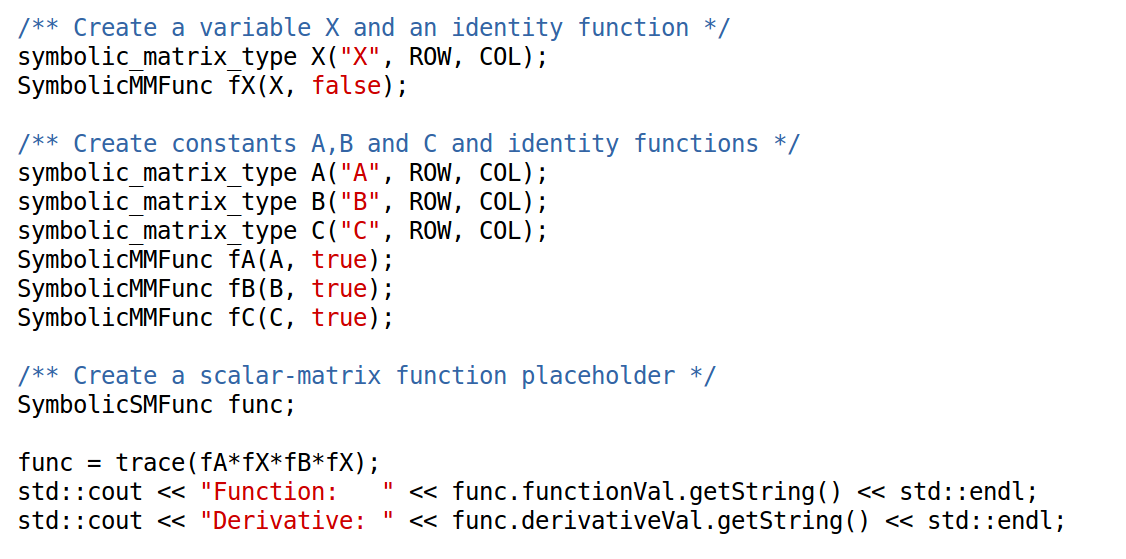
\includegraphics[width=0.8\textwidth]{example1.png}
\end{figure}
\onslide<2> {
The derivative of the scalar-matrix function is:
\begin{figure}[p]
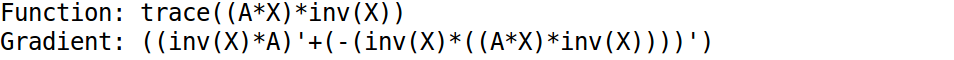
\includegraphics[width=0.8\textwidth]{result1.png}
\end{figure}

The result is in Matlab syntax. 
}
\end{frame}


\begin{frame}
\frametitle{Compute in command line}
This is an Symbolic Matrix Differentiation Calculator which takes the expression 
input in command line and then output the derivative. The examples are $\color{m1}trace(A\times X) + trace(B \times X^{-1})$ 
and $\color{m1}logdet(A\times X \times \times B \times X)$. 
\begin{figure}[p]
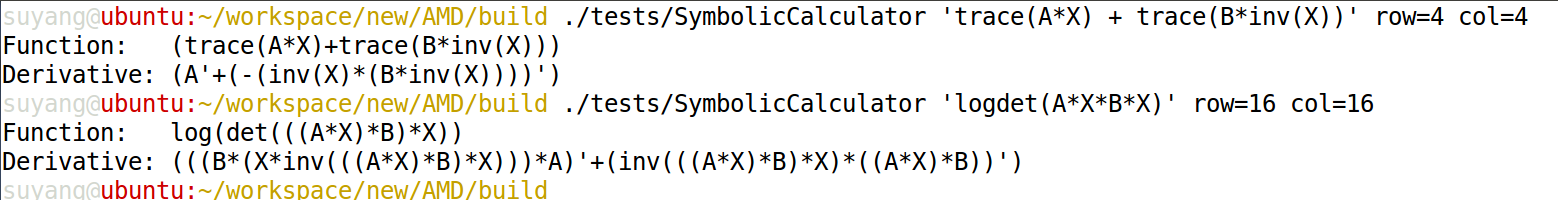
\includegraphics[width=1.0\textwidth]{example2.png}
\end{figure}
\end{frame}

\section{Taylor Expansion}
\begin{frame}
\frametitle{Taylor expansion}
Recall that for a scalar-scalar function the Taylor expansion of a
function $f$ around a value $x_0$ looks like:
$$\color{m1}
f(x) = f(x_0)+(x-x_0)f'(x_0)+\frac{1}{2}(x-x_0)^2f''(x_0)+\frac{1}{3!}(x-x_0)^3f'''(x_0)+\cdots
$$
For a vector valued function $f'(\vx_0)$ is a vector and $f''(\vx_0)$
is a matrix, so the Taylor expansion looks like
$$\color{m1}
f(\vx) = f(\vx_0)+(\vx-\vx_0)^{\top}f'(\vx_0)+\frac{1}{2}(\vx-\vx_0)^{\top} f''(\vx_0)(\vx-\vx_0)+\cdots
$$
The third derivative here is a 3-dimensional tensor, and it's a bit
unclear what the best way to continue the expansion is.  For
scalar-matrix functions it's even messier.
\end{frame}

\begin{frame}
\frametitle{Taylor expansion for scalar-matrix functions}
For a matrix-matrix function like $\color{m1} F(\mX)=(\mX+\mI)^{-1}$ with $\mX_0=0$
we can pretend $\color{m1}\mX$ is a scalar and get
$$\color{m1}
(\mX+\mI)^{-1}= \mI+\mX-\mX^2+\mX^3+\cdot
$$
Thus for a scalar-matrix function like $\color{m1}f(\mX)=\trace((\mX+\mI)^{-1})$ we can
write the Taylor expansion as
$$\color{m1}
\trace((\mX+\mI)^{-1})= \trace(\mI)+\trace(\mX)-\trace(\mX^2)+\trace(\mX^3)+\cdot,
$$
and although we do not explicitly compute $\color{m1}f'(\mX), f''(\mX), f'''(\mX),\ldots$
this computes the individual terms of the Taylor expansion efficiently.
\end{frame}

\begin{frame}
\frametitle{Taylor expansion for logdet(X)}
We use these matrix differentition rules to compute the Taylor expansion around the point $\color{m1}\mX_0$
\begin{equation}
\begin{split}
\color{m1} \logdet(\mX) &= \color{m1}\logdet(\mX_0) + \trace((\mX-\mX_0)\mX_0^{-1}) \\
         &\color{m1}+\frac{1}{2!}\trace(-(\mX-\mX_0)\mX_0^{-1}(\mX-\mX_0)\mX_0^{-1}) \\
         &\color{m1}+ \frac{1}{3!}\trace(2(\mX-\mX_0)\mX^{-1}(\mX-\mX_0)\mX^{-1}(\mX-\mX_0)\mX^{-1}) \cdots
\end{split}
\end{equation}
\end{frame}

\begin{frame}
We notice that we can compute each part of the Taylor series iteratively:
\begin{equation}
\color{m1}f_0(\vx) = \logdet(\mX_0) 
\end{equation}
\begin{equation}
\color{m1}f_1(\vx) = \trace((\mX-\mX_0)(f_0'(\vx))^{T})
\end{equation}
\begin{equation}
\color{m1}f_2(\vx) = \trace((\mX-\mX_0)(f_1'(\vx))^{T})
\end{equation}
\begin{equation}
\color{m1}f_3(\vx) = \trace((\mX-\mX_0)(f_2'(\vx))^{T})
\end{equation}
The previous equation $\color{m1}(1)$ can be computed as:
$$
\color{m1} \logdet(\mX) = f_0(\vx) + f_1(\vx) + \frac{1}{2!}f_2(\vx) + \frac{1}{3!}f_3(\vx) \cdots
$$
\end{frame}

\begin{frame}
\frametitle{Taylor expansion for logdet(X) cont} 
Here is the code to compute nth order derivative iteratively.
\begin{figure}[p]
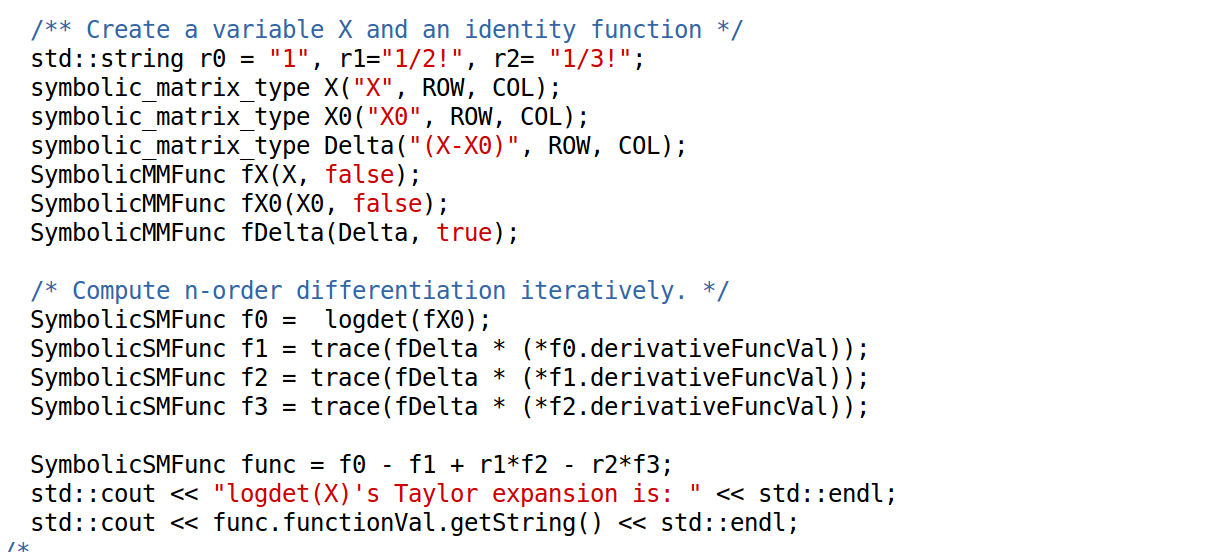
\includegraphics[width=0.8\textwidth]{taylorCode.png}
\end{figure}
\onslide<2> {
This figure is the output for nth order derivative.
\begin{figure}[p]
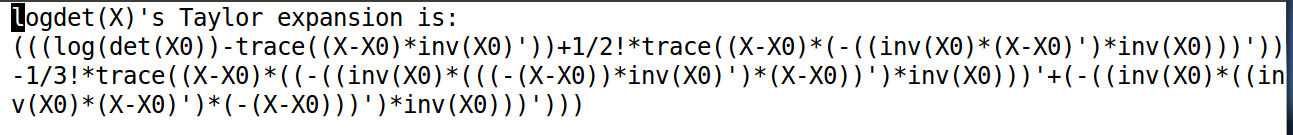
\includegraphics[width=1.0\textwidth]{taylor.png}
\end{figure}
}
\end{frame}






\end{document}
